\chapter{Sviluppo e implementazione}
\label{cha:sviluppo_implementazione}

Il prototipo realizzato con Figma, per quanto semplice, ha permesso di indirizzare da subito i passaggi dello sviluppo: realizzazione del codice del front-end progettato e successiva implementazione dello sviluppo del back-end.

Successivamente viene descritto l'effettivo funzionamento dell'app, con relative illustrazioni, prestando attenzione anche ad architettura e tecnologie utilizzate.

\section{Tecnologie utilizzate}
\label{sec:tecnologie}

Di seguito sono presentate brevemente le varie tecnologie utilizzate per l'implementazione di VolleyVisionAI.


\subsection{Node.js}
\begin{wrapfigure}{r}{0.33\textwidth}
    \centering
    
\includegraphics[scale=0.17]{nodejs.png}
    \caption{Logo NodeJS}
\end{wrapfigure}
    
Node.js è un runtime system in JavaScript orientato agli eventi e completamente Open-Source. Garantisce performance e prestazioni elevate, basandosi sul motore JavaScript V8 di Google Chrome. Node.js è particolarmente valorizzato per il suo accesso a \textit{Node Package Manager}. NPM è un gestore di pacchetti predefinito per l'ambiente di runtime JavaScript Node.js, nonchè il più grande ecosistema di librerie open source al mondo. Questo permette agli sviluppatori di utilizzare soluzioni già pronte condivise dalla community, accelerando le fasi di programmazione e garantendo sicurezza e solidità del codice.


\subsection{React.js}
\begin{wrapfigure}{r}{0.33\textwidth}
    \centering
    \vspace{-15px}
    
\includegraphics[scale=0.15]{react.png}
    \caption{Logo ReactJS}
\end{wrapfigure}
    
ReactJS è una libreria JavaScript, anche essa Open Source, sviluppata da Meta per la costruzione di interfacce utente, particolarmente utilizzato per complesse \textit{User-Interface} e applicazioni a pagina singola. Questa libreria è largamente utilizzata ed apprezzata per il suo vasto ecosistema, che include strumenti come \textit{React Developer Tools} e \textit{Create React App}. Per lo sviluppo della mia app ho adottato proprio quest'ultimo che utilizza \textit{Node.js} e \textit{NPM}, permettendomi di avviare un progetto React in maniera semplice e veloce. Inoltre React è una libreria che utilizza una struttura basata su componenti, che permettono di creare interfacce riutilizzabili e modulabili


\subsection{Figma}
\begin{wrapfigure}{r}{0.33\textwidth}
    \centering
    \vspace{-20px}
    
\includegraphics[scale=0.20]{figma.png}
    \caption{Logo Figma}
\end{wrapfigure}
    
Figma è uno strumento di design e grafica vettoriale utilizzato per la creazione di mockup e prototipi. Figma si distingue per essere un applicativo Web, ma che permette comunque soluzioni desktop e mobile. L'obiettivo di Figma è quello di permettere la creazione di design facendo particolare attenzione a \textit{User Experience} e \textit{User Interface}, permettendo inoltre la collaborazione \textit{realtime} tra utenti. Figma è stato fondamentale in fase di analisi e progettazione, poichè mi ha permesso di avere un prototipo dell'app prima dell'implementazione effettiva.

\pagebreak


\subsection{Uvicorn}
\begin{wrapfigure}{r}{0.33\textwidth}
    \centering
    \vspace{-10px}
    
\includegraphics[scale=0.15]{uvicorn.png}
    \caption{Logo Uvicorn}
\end{wrapfigure}

Uvicorn è un server ASGI (Asynchronous Server Gateway Interface), ideato e progettato per eseguire applicazioni web asincrone in Python, in maniera leggera e veloce. La sua architettura asincrona lo rende ottimale per lavorare con framework moderni come \textit{FastAPI} e \textit{Starlette}, permettendogli di gestire un elevato numero di richieste simultaneamente senza problemi. La tecnologia HTTP/2 e WebSocket sono supportate da Uvicorn, rendendolo ideale per applicazioni realtime. Uno dei motivi principali per cui ho scelto di utilizzare un server meno conosciuto come questo è la sua compatibilità con \textit{FastAPI}. Queste tecnologie combinate tra loro, mi permettono di avere un server Back-End veloce ma soprattutto scalabile. 


\subsection{FastAPI}
\begin{wrapfigure}{r}{0.33\textwidth}
    \centering
    
\includegraphics[scale=0.18]{fastapi.png}
    \caption{Logo FastAPI}
\end{wrapfigure}
    

FastAPI è un framework web progettato per creare API in Python. Il framework si basa su standard quali, OpenAPI e JSON Schema, che gli permettono di generare documentazione interattiva in maniera completamente automatica. Come descritto in precedenza, FastAPI utilizza \textit{Uvicorn} come server ASGI a cui delega la gestione delle richieste. Questo permette di avere un'applicazione estremamente veloce, una caratteristica fondamentale per le applicazioni web moderne. Inoltre, ho optato per questa soluzione in quanto FastAPI ha una documentazione chiara e completa, che mi ha permesso di utilizzare il framework senza problemi. 


\subsection{YOLOv9 }
\begin{wrapfigure}{r}{0.33\textwidth}
\centering
\vspace{-5px}

\includegraphics[scale=0.4]{Yolo.png}
\caption{Logo Ultralytics}
\end{wrapfigure}

YOLOv9 è un modello di \textit{object-detection} sviluppato da Ultralytics. Questa ultima versione della famiglia YOLO (You Only Look Once), è una delle soluzioni più avanzate presenti al momento sul mercato. YOLOv9 viene presentato in 5 varianti principali che si distinguono per la loro complessità. In particolare differiscono per la quantità di parametri di cui il modello dispone, ovvero, le varianti più complesse faranno rilevamenti più precisi a discapito di una maggiore richiesta computazionale. Nel contesto della mia Web App, avere la possibilità di scegliere quale tra le soluzioni fosse la più adatta al progetto mi ha fatto scegliere YOLOv9 come soluzione.

\subsection{OpenCV}
\begin{wrapfigure}{r}{0.33\textwidth}
\centering
\vspace{-10px}

\includegraphics[scale=0.1]{OpenCv.png}
\caption{Logo OpenCV}
\end{wrapfigure}

OpenCV, acronimo di Open Source Computer Vision, è una libreria per la visione artificiale e l'elaborazione delle immagini. E' scritta in C++ ma ha anche altre interfacce, una di queste è in Python, che ho utilizzato nel mio progetto. Gli strumenti messi a disposizioni da OpenCV vengono integrati con modelli, nel mio caso YOLOv9, utilizzando i loro risultati per elaborare specifiche grafiche video. La libreria è stata scelta per la sua documentazione e versatilità, ideale per uno sviluppatore che come me è alle prime armi con il mondo AI.  
% YOLOv9 è un modello di \textit{object-detection} sviluppato da Ultralytics. Questa ultima versione della famiglia YOLO (You Only Look Once), è una delle soluzioni più avanzate presenti al momento sul mercato. YOLOv9 viene presentanto in 5 varianti principali che si distinguono per la loro complessità. In particolare differiscono per la quantità di parametri di cui il modello dispone, ovviamente una variante più complessa farà rilevamenti più precisi a discapito di una maggiore richiesta di risorse. Nel contesto della mia Web App, avere la possibilità di scegliere quale tra le soluzioni fosse la più adatta al progetto mi ha fatto scegliere Yolov9 come soluzione.

\pagebreak

\section{Implementazione}
\label{sec:implementazione}

L'implementazione rispetta le premesse definite nelle fasi di analisi e progettazione, concentrandosi sul mantenere una \textit{User Interface} pulita e un'architettura solida e scalabile.
Attualmente la Web App non è ospitata pubblicamente (Deploy) in quanto ancora in fase di sviluppo.
Lo sviluppo principale è stato lato Front-End implementando tutte le funzionalità definite nel capitolo \ref{cha:analisi_progettazione}. Per l'avvio ho utilizzato \textit{create-react-app} necessario a creare l'ambiente di sviluppo. Questo configura in maniera autonoma, tramite l'utilizzo di  \textit{webpack-dev-server}, un server di sviluppo basato su \textit{Node.js} che serve un interfaccia \textit{React} sul browser locale offrendo così un ambiente caratterizzato dal \textit{live reloading}, utile per vedere i cambiamenti apportati nel codice in \textit{real time}. 
La componente \textit{UnifiedContext.js} è stata utilizzata per centralizzare la gestione dello stato della Web App. In questo modo vengono salvati i dati inseriti dall'utente durante l'utilizzo dell'applicazione, come atleti, azioni, shortcut attivati ed eventi taggati. 
Nel Front-End sono implementate tutte le funzionalità ad eccezione di quelle che richiedono maggiori risorse computazionali (es la manipolazione di video o l'applicazione di modelli AI) in quanto delegate tramite API ad un server \textit{Back-End} esterno.
Questo approccio \textit{Multi Server} è stato pensato per alleggerire il lavoro lato client e garantire una maggiore scalabilità in ottica degli sviluppi futuri dell'applicazione.
Questa componente server Back-End è stata sviluppata in Python tramite il pacchetto Python \textit{FastAPI} supportato a sua volta dal server ASGI \textit{Uvicorn}. La scelta di questo Framework (vedi \ref{sec:tecnologie}) ha permesso di creare API in maniera semplice.
L'implementazione con FastAPI gestisce due funzionalità principali: la creazione di videoclip e l'applicazione di modelli AI. Nella prima viene utilizzato il modulo \textit{moviepy} che permette l'\textit{editing} di video. Mentre, per la seconda si è scelto il modello YOLOv9 nella variante YOLOv9c in quanto adatta alla complessità di object-detection che necessita la Web App. L'uso del modello è delegato alla libreria OpenCV con la sua implementazione Python, che permette la gestione grafica dei risultati. Per l'identificazione dei singoli atleti in campo è stato utilizzato l'algoritmo \textit{SORT} (Simple Online and Realtime Tracking), che ha permesso di mantenere l'identità dei singoli per tutta la durata del video.  

\subsection{Architettura}
\label{sec:architettura}

L'architettura di sviluppo della Web App è rappresentata in figura \ref{fig:architettura_app}.

\begin{figure}[h]
    \centering
    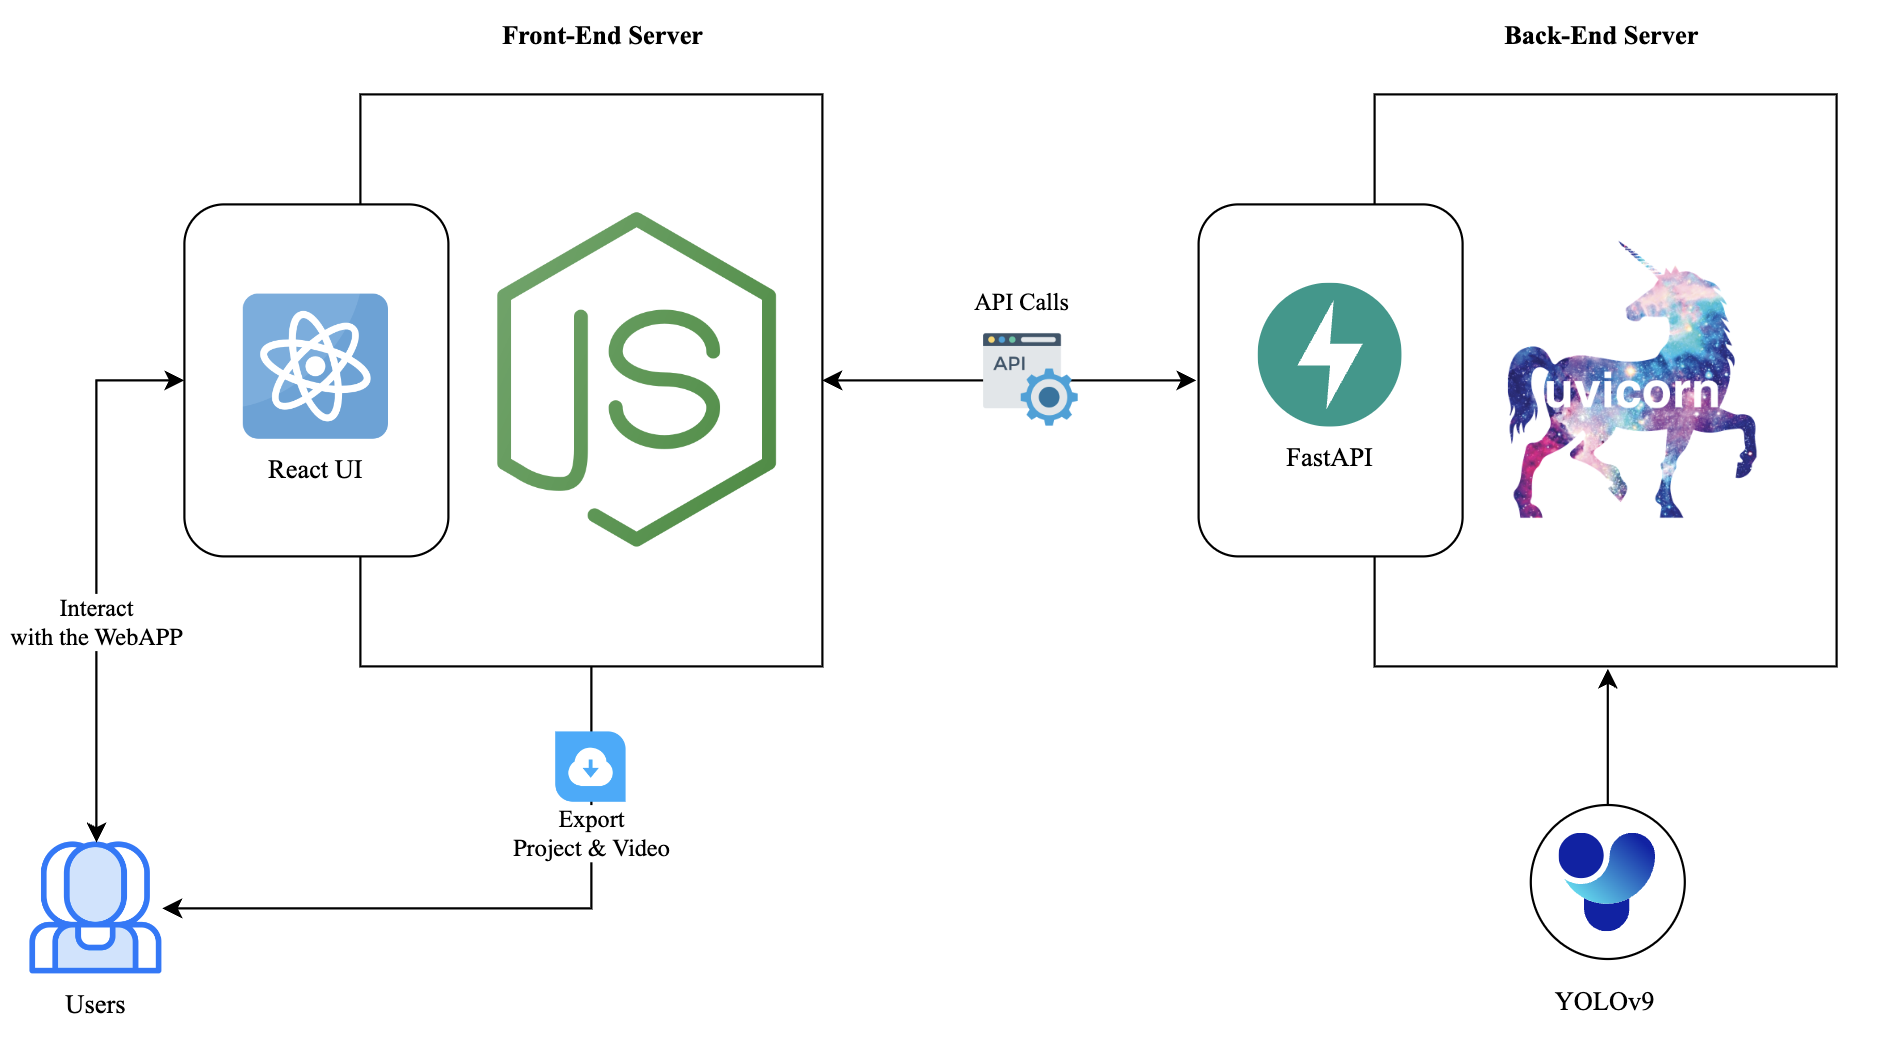
\includegraphics[width=1.02\textwidth]{Architettura.png}
    \caption{Architettura Web App}
    \label{fig:architettura_app}
\end{figure}







\section{UI e Funzionamento Web App}
\label{sec:funzionamento}

Nel seguente paragrafo vengono presentate le funzionalità dell'app mantenendo un ordine logico di navigazione.


\subsection{Menu iniziale}
\label{sec:menu_iniziale}

Il menu iniziale è la prima schermata a cui si accede lanciata la Web App. Questo ha la funzione di guidare l'utente attraverso le modalità base dell'applicazione. Il menu presenta il logo della Web App con le due principali opzioni d'uso: \textit{Manual} ed \textit{AI}.


\begin{figure}[h]
    \centering
    \frame{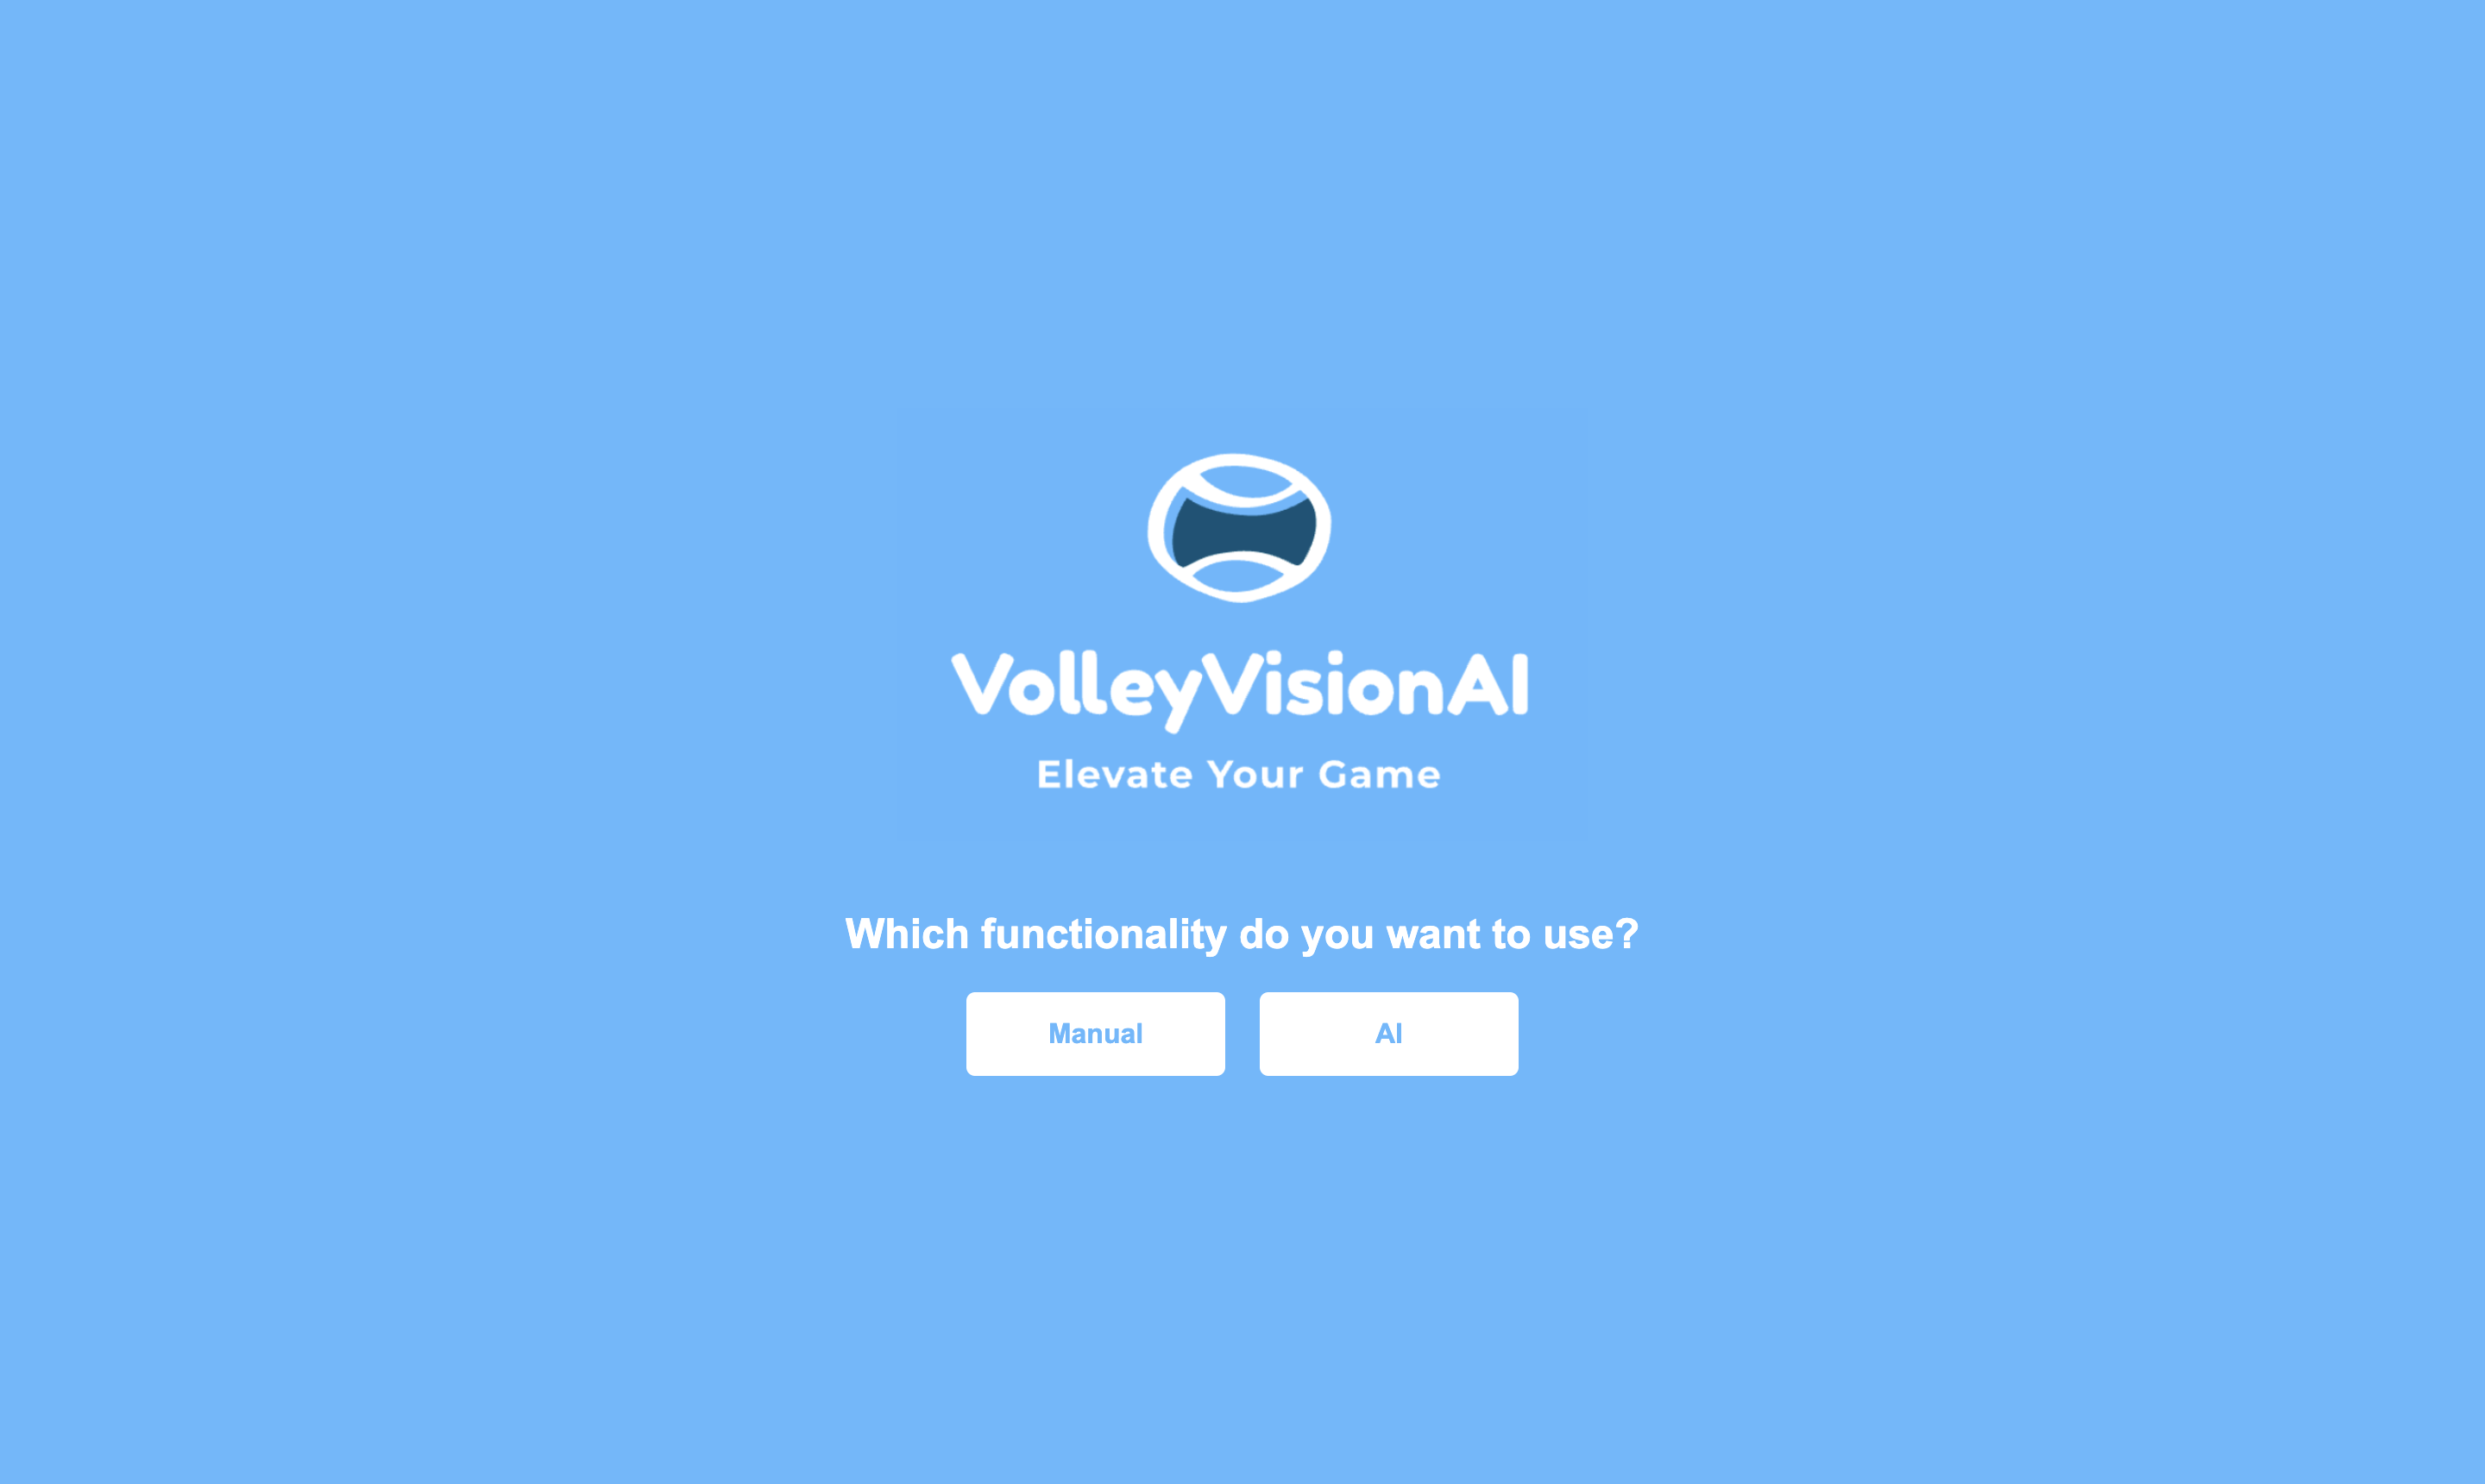
\includegraphics[scale=0.22]{Menu_iniziale.png}}
    \caption{Menu iniziale}
    \label{fig:bot-menu-iniziale}
\end{figure}

\noindent Ciascuna di queste opzioni porta ad una schermata con le relative funzionalità.

\begin{itemize}
    \item \textbf{Manual}: una volta effettuata questa scelta, l'utente dovrà decidere se creare un nuovo progetto o caricare uno già esistente. Nel primo caso l'applicazione chiederà di inserire i nomi degli atleti e le azioni che vuole raccogliere. Essendo la Web App verticale per lo sport della pallavolo, sono già presenti i fondamentali principali come battuta, attacco, difesa, alzata e muro. Questo avviene per facilitare la configurazione, viene comunque permesso di aggiungere ulteriori etichette. Nel caso dell'importazione di un progetto già esistente, la risposta sarà di individuare sul \textit{file-system} il file di un progetto precedentemente esportato. Effettuato questo setup di istruzione, l'applicazione prosegue con la schermata di \textit{Analisi Manuale}.
    
    \item \textbf{AI}: questa modalità richiede di caricare il video da analizzare, specificando il tipo di riconoscimento desiderato, \textit{Ball Tracking} o \textit{Players Recognition}. Dato che questa operazione è delegata al back-end, l'UI mostrerà un messaggio di attesa finchè il video non è stato elaborato, per poi passare alla schermata di \textit{Analisi AI}.
    
\end{itemize}


\noindent In ciascuna delle due opzioni è permesso, in qualsiasi momento, di tornare al menu iniziale attraverso il bottone dedicato.



\subsection{Analisi Manuale}
\label{subsec:funzionalita_manual}

La funzionalità di \textit{Analisi Manuale} consente all'utente di eseguire operazioni manuali come il \textit{tagging} degli eventi, il disegno su video e la creazione di videoclip. La schermata è caratterizzata da quattro elementi principali che permettono all'utente di svolgere le funzionalità descritte in precedenza. Inoltre l'interfaccia usa colori in maniera intelligente per differenziare i vari elementi migliorando la \textit{User Experience} dell'utente finale.

Seguendo una logica di navigazione, le principali funzionalità vengono descritte di seguito.



\newpage

\subsubsection{Add Shortcut}
\begin{wrapfigure}{r}{0.55\textwidth}
    \centering
    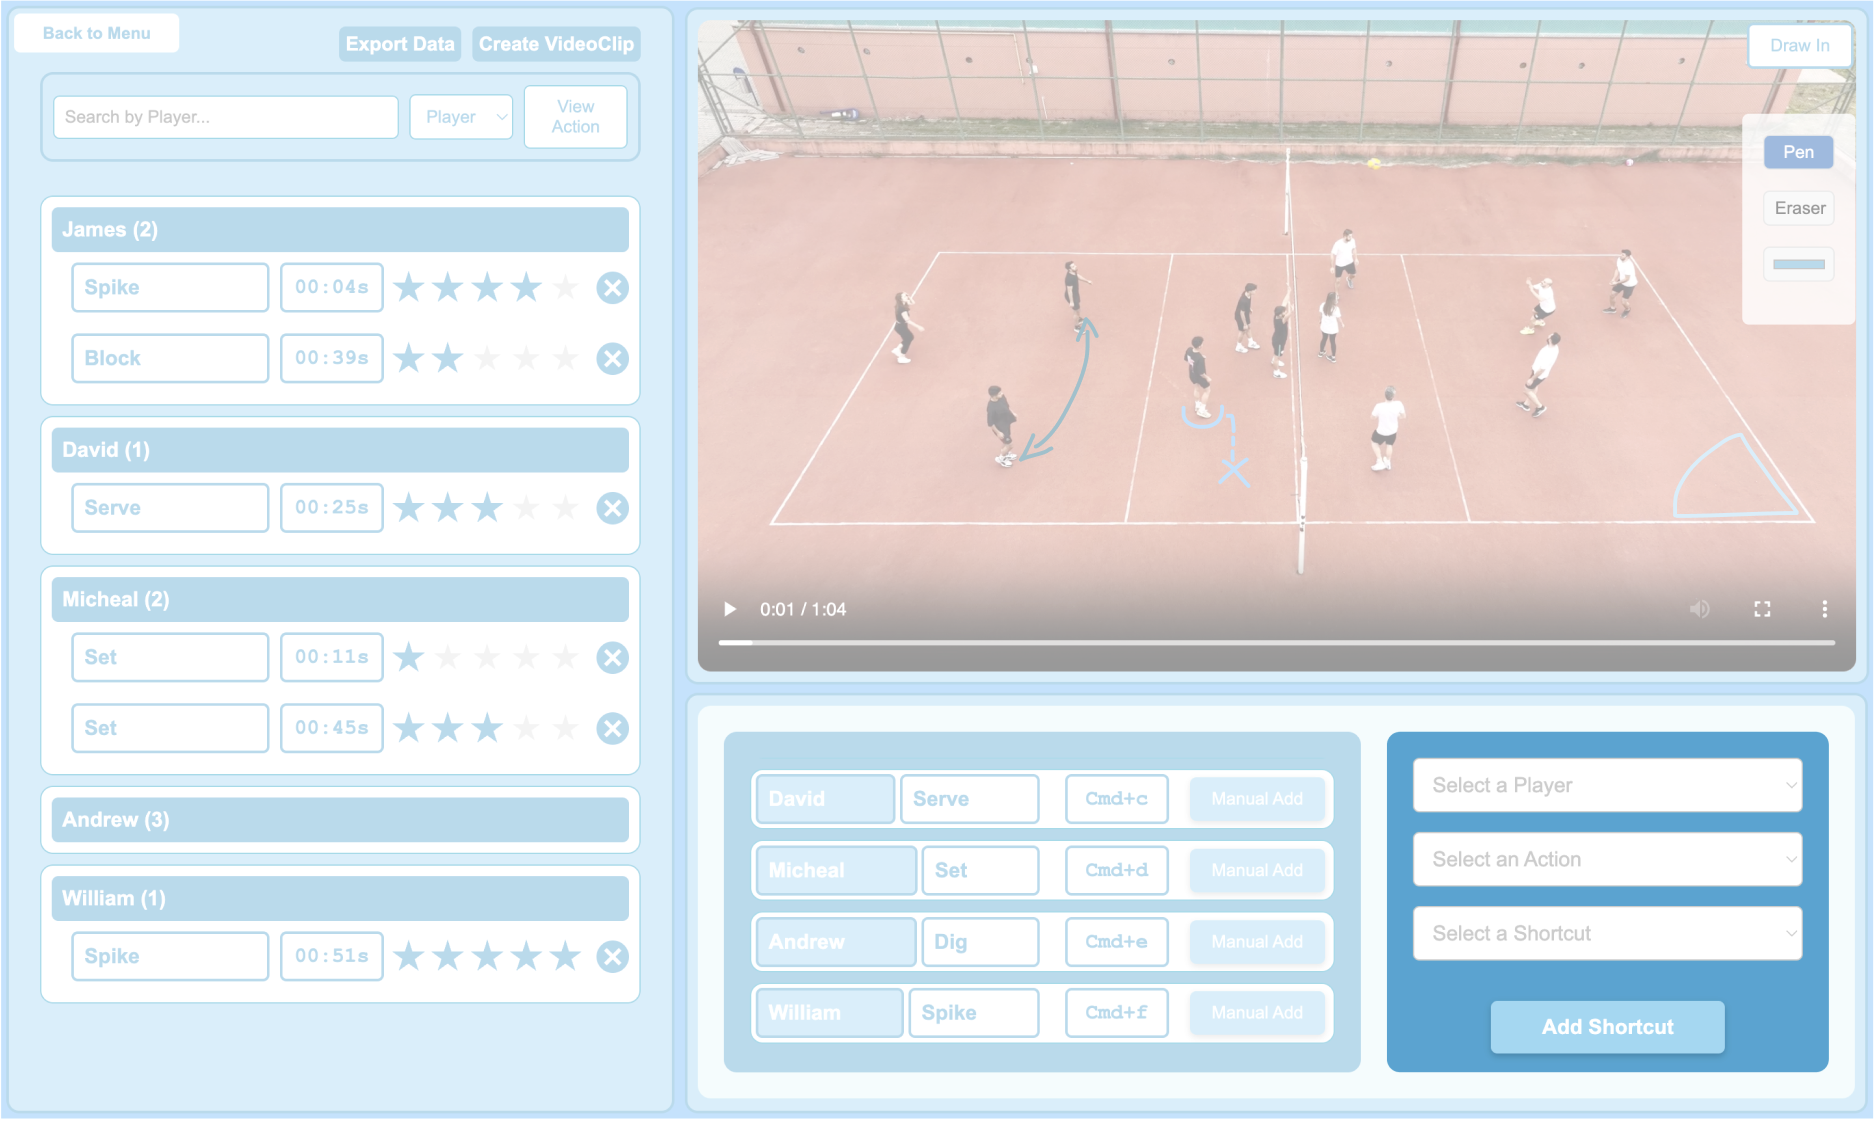
\includegraphics[width=\linewidth]{add_listener.png}
    \captionof{figure}{Add Shortcut}
    \label{fig:add_listener}
\end{wrapfigure}

posto in basso a destra, al di sotto del \textit{VideoPlayer}, si trova un contenitore suddiviso in due componenti di cui l'\textit{Add Shortcut} è quello sulla destra. Questo permette di creare nuovi shortcut personalizzati che servono durante la fase di \textit{Event Tagging}. In particolare è composto da tre menu a tendina che permettono di selezionare l'atleta, l'azione e il comando rapido (shortcut) che si vuole creare. La configurazione dei parametri viene confermata al click sulla voce  "Add Shortcut" sottostante. Naturalmente ogni comando rapido può essere assegnato ad un solo tipo di evento. Se ne viene inserito uno già presente allora l'applicazione rimuove il precedente e lo assegna alla nuova funzionalità scelta.

\subsubsection{Shortcut Summary}
\begin{wrapfigure}{r}{0.55\textwidth}
    \centering
    \vspace{-0.4cm} % Abbassa l'immagine
    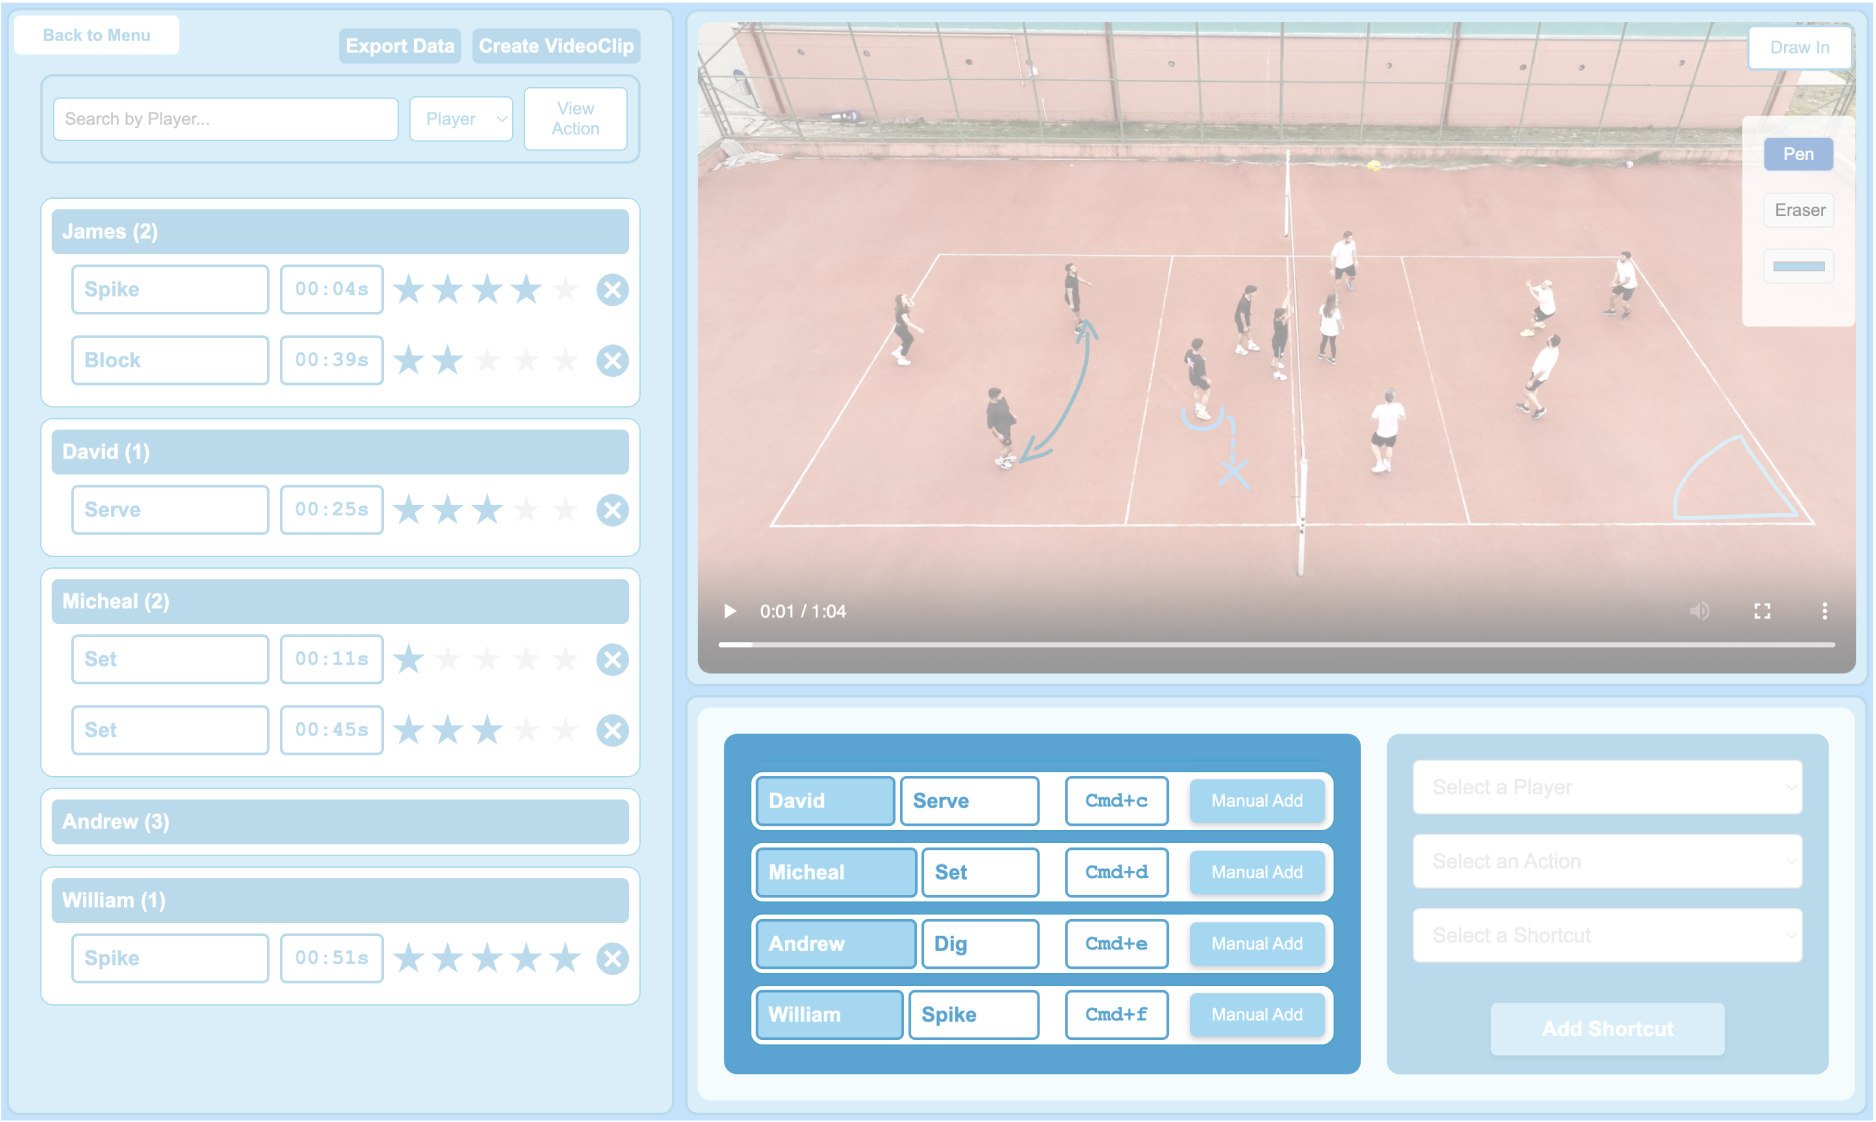
\includegraphics[width=\linewidth]{Summary.png}
    \captionof{figure}{Enabled Shortcut}
    \label{fig:Enabled_shortcut}
\end{wrapfigure}

Creato un qualsiasi shortcut, l'interfaccia presenta, all'interno dello stesso contenitore di \textit{Add Shortcut} ma sulla sua sinistra, il pannello \textit{Shortcut Summary}. La funzione di questo componente permette di tenere traccia degli shortcut creati, rendendoli visualizzabili in una lista che per ognuno ne definisce giocatore, azione e comando rapido. Per migliorare ulteriormente la \textit{User Experience}, ogni shortcut è affiancato da un bottone "Manual Add" che permette ad utenti che non sanno utilizzare gli shortcut da tastiera, di poter comunque utilizzare questa funzionalità dell'app.

\subsubsection{Tagged Events}
\begin{wrapfigure}{r}{0.55\textwidth}
    \centering
    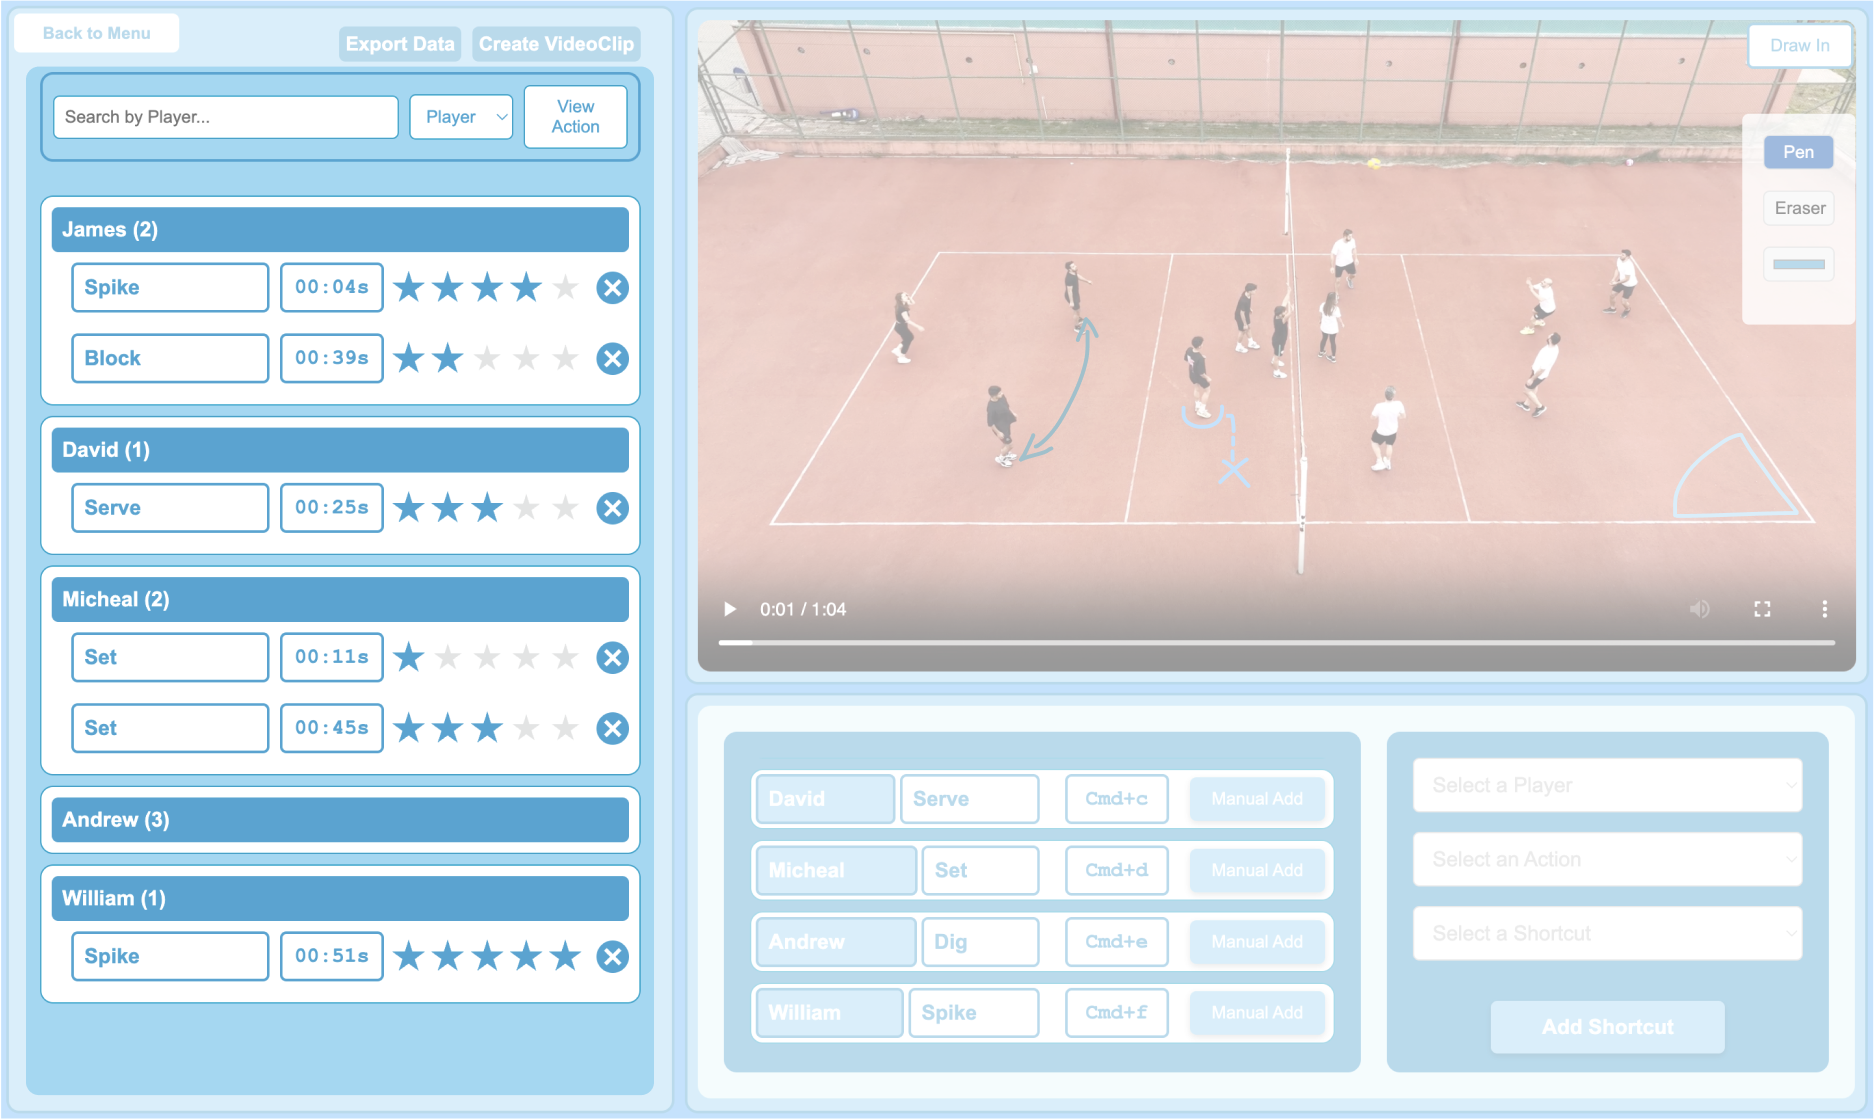
\includegraphics[width=\linewidth]{activated_shortcut.png}
    \captionof{figure}{Tagged Events}
    \label{fig:activated_shortcut}
\end{wrapfigure}

Sulla sezione sinistra dello schermo troviamo uno dei componenti fondamentali della Web App. Una volta che uno shortcut viene attivato, sia tramite comando rapido da tastiera che tramite il bottone "Manual Add" nel componente \textit{Shortcut Summary}, viene visualizzato qui dentro. Il componente è composto da una Search Bar che permette di cercare determinati eventi, selezionando anche se filtrarli in base al giocatore o all'azione. Nell'area sottostante sono invece elencati tutti gli eventi taggati in una lista suddivisa in gruppi. Gli eventi vengono raggruppati in base alla scelta dell'utente, può infatti decidere di visualizzarli in gruppi in base all'azione o in base al giocatore grazie al bottone che cambia tra "View by Action" e "View by Player". L'utente può cambiare questo tipo di visualizzazione in ogni momento. Ad ogni evento taggato corrispondono inoltre altre 2 variabili: il minutaggio e la valutazione. Il primo rappresenta il momento in cui è avvenuto l'evento taggato, dando la possibilità all'utente di cliccarlo per spostare il video a quel preciso istante. Il secondo invece è un componente composto da 5 stelle, inizialmente chiare, che sono utilizzabili dall'utente per dare valutazioni agli eventi taggati. È sempre disponibile, nel caso di uno shortcut attivato per errore, la possibilità di cancellarlo tramite un pulsante X presente accanto ad ognuno.

\subsubsection{Video Player}
\begin{wrapfigure}{r}{0.55\textwidth}
    \centering
    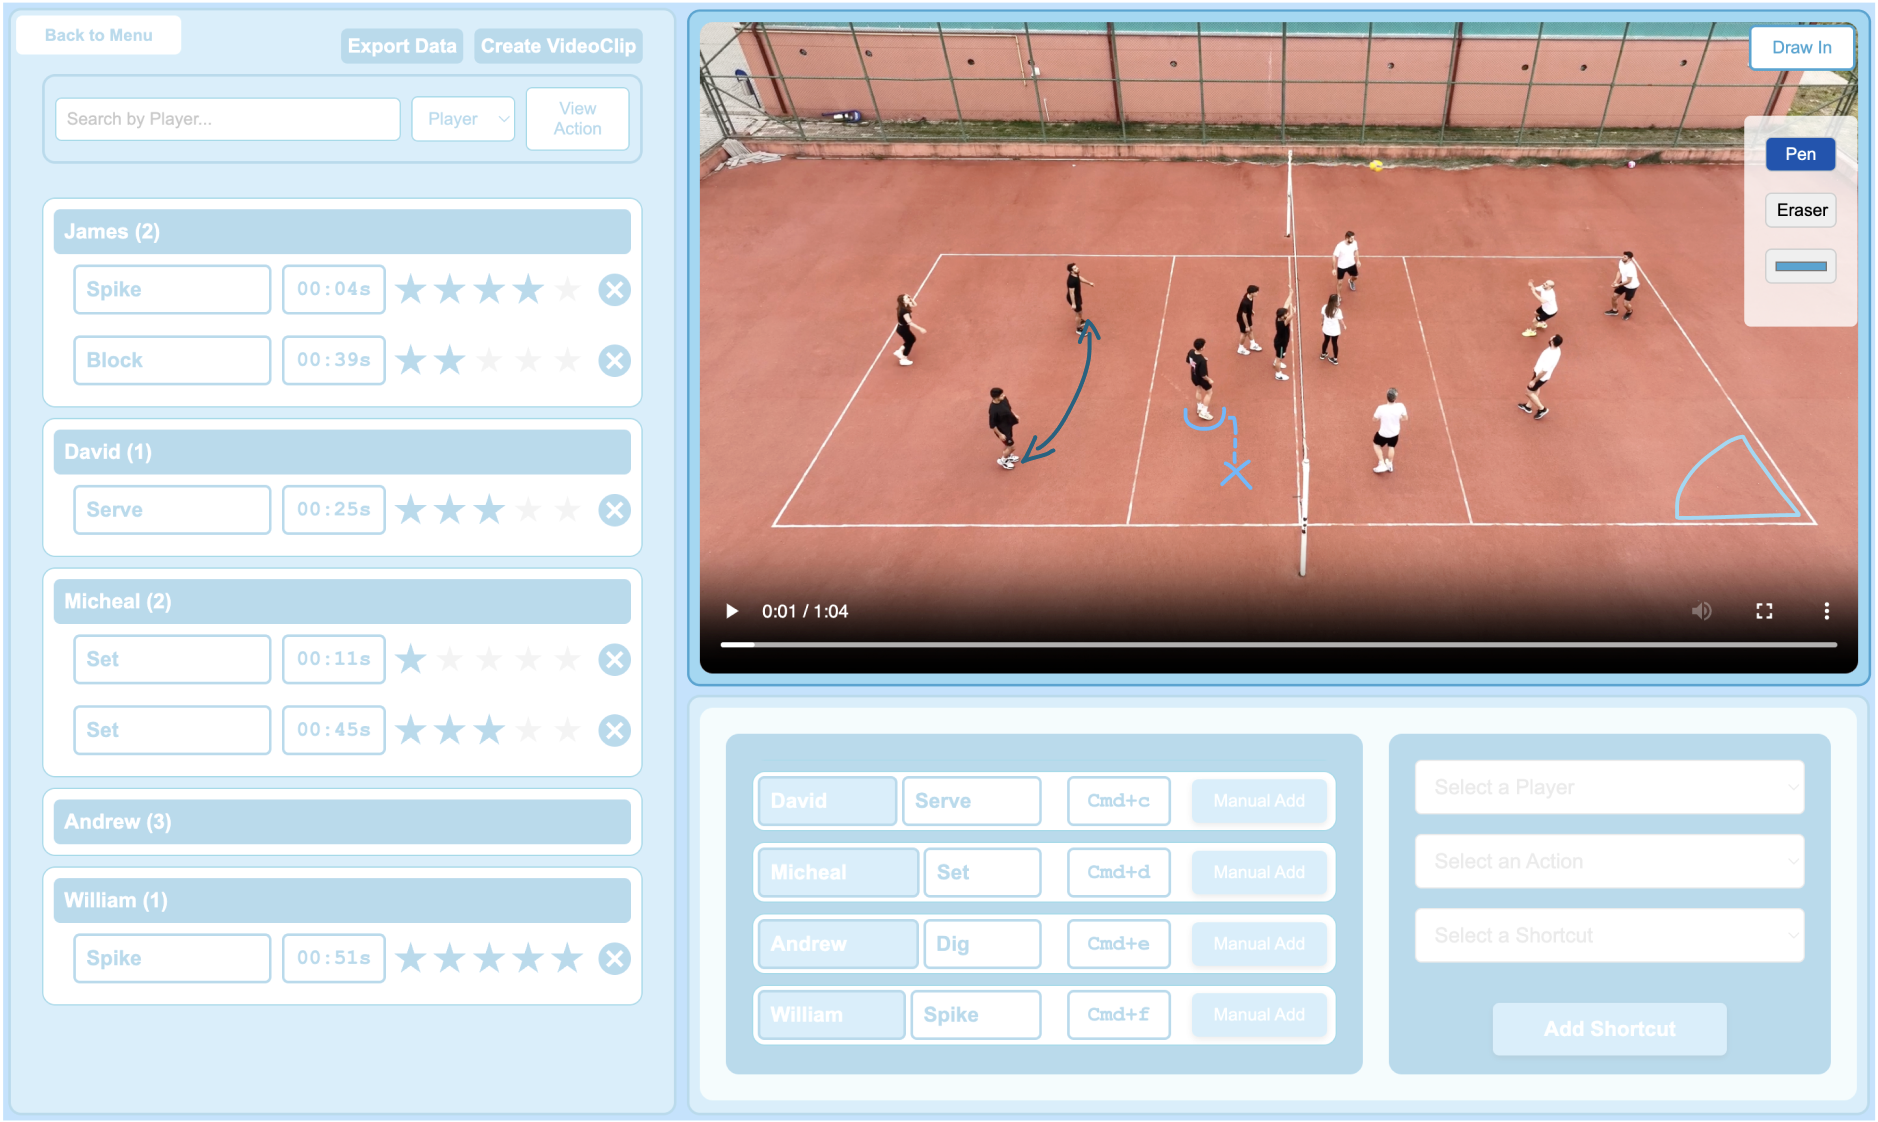
\includegraphics[width=\linewidth]{video_player.png}
    \captionof{figure}{Video Player}
    \label{fig:video_player}
\end{wrapfigure}

In alto a destra, sopra al contenitore di \textit{Shortcut Summary} e \textit{Add Shortcut}, è collocato il componente principale di VolleyVisionAI, ovvero il \textit{Video Player}. Questa sezione mostra all'utente il video caricato permettendo di interagire con esso come un normale \textit{Player Video}, consentendo quindi di controllare la riproduzione, mettere in pausa, avanzare o tornare indietro nel video, e regolare il volume.  Inoltre qui viene implementata la funzionalità di \textit{Drawing} che permette di disegnare sul video. In particolare, tramite il bottone "Draw In" l'utente può attivare la funzionalità di disegno che implementa una dashboard molto semplice.  Quest'ultima permette all'utente di scegliere se usare penna per disegnare o gomma per cancellare. Inoltre è possibile anche scegliere quello che è il colore del tratto, così da aiutare l'utente nel diversificare le sue annotazioni. Ogni volta che l'utente riclicca il pulsante "Draw In" la dashboard e le annotazioni scompariranno, rendendo il video pulito in caso di future annotazioni.

\subsubsection{Export \& Create Videoclip}

Nell'area sovrastante al componente \textit{Tagged Events}, precisamente sopra alla search bar, sono collocati due pulsanti di seguito descritti:
\begin{itemize}
    \item \textbf{Export Project:} consente di esportare il progetto, permettendo all'utente di salvarlo in locale e riutilizzarlo in futuro. In realtà questo bottone non è l'unico che permette di esportare il progetto, infatti se l'utente decide di tornare al menu principale gli verrà richiesto se vuole esportare il progetto prima di abbandonare la pagina. Il progetto viene esportato scaricando sul dispositivo dell'utente un file JSON contenente lo stato dell'app fino a quel momento.
    \item \textbf{Create Videoclip:} consente di creare videoclip in maniera automatica elaborando gli eventi taggati in precedenza. In particolare viene richiesto all'utente di selezionare la durata media delle clip che andranno a comporre il video. Questa scelta viene presentata come una barra scorrevole con estremi 1s e 15s, così da lasciare all'utente margine di scelta. Successivamente l'utente cliccando il bottone "Create Clip" viene messo in attesa finchè il Back-End non ha elaborato il video. Ogni singola clip è caratterizzata dal testo "Giocatore - Azione" di quell'evento taggato. Una volta terminato il processo, la Web App scarica automaticamente il video risultante sul dispositivo dell'utente.
\end{itemize}

\noindent Come scritto in precedenza, infine, è presente il pulsante "Back to Menu" in alto a sinistra che permette all'utente di tornare al menu principale in qualsiasi momento.
% . Quello  di Esportare il progetto, permettendo all'utente di salvare in locale il progetto e poi riutilizzarolo nel futuro. 
% Appena sopra alla Search Bar troviamo 2 pulsanti, uno per esportare il progetto e l'altro per creare un videoclip. Il primo pulsante permette di salvare il progetto corrente come un file JSON, mentre il secondo consente di creare un videoclip a partire dagli eventi taggati. Questo componente è progettato per semplificare il processo di salvataggio e condivisione dei progetti, consentendo all'utente di esportare i risultati in modo rapido e intuitivo.
\pagebreak
\clearpage


\subsection{Analisi AI}
\label{subsec:funzionalita_ai}

L'\textit{Analisi AI}, seppur ancora in stato embrionale, rappresenta la funzionalità più innovativa dell'app. 

Inizialmente una volta scelta questa modalità viene richiesto all'utente di caricare sull'app il video che vuole analizzare e il tipo di analisi AI che vuole applicare.
Una volta inseriti i dati richiesti, tramite il bottone "Apply AI", l'utente viene messo in una schermata d'attesa caratterizzata da una scritta centrale  "Applying Model", in modo tale da far capire all'utente che VolleyVisionAI sta elaborando il risultato.
Una volta che l'output video è stato generato, l'utente viene portato all'effettiva pagina di Analisi AI.
Questa pagina differisce in base al tipo di analisi scelta dall'utente, in particolare se ha scelto di riconoscere la traiettoria della palla o identificare i singoli giocatori.

\subsubsection{Ball Trajectory}
\begin{wrapfigure}{r}{0.55\textwidth}
    \centering
    \vspace{-0.4cm}
    \includegraphics[width=\linewidth]{ball_recognition.png}
    \captionof{figure}{Ball Trajectory}
    \label{fig:ball_trajectory}
\end{wrapfigure}

Questa funzionalità utilizza il modello YOLOv9c per riconoscere la palla. Vengono impostati in particolare 2 parametri: \textit{confidence} e \textit{object-type}. Per questo tipo di analisi impostiamo la confidenza a 0.6 e il tipo di oggetto a "32". Queste specifiche servono rispettivamente per evitare falsi positivi e per specificare al modello che deve riconoscere una palla. Successivamente i risultati di Yolo vengono utilizzati da OpenCV per rappresentare graficamente la traiettoria. In particolare, vengono presi gli ultimi 30 frame della palla e per ognuno di essi viene disegnato un punto giallo. Questo insieme di punti creano visivamente la traiettoria della palla.

\subsubsection{Players Identification}
\begin{wrapfigure}{r}{0.55\textwidth}
    \centering
    \vspace{-0.5cm}
    \includegraphics[width=\linewidth]{player_recognition.png}
    \captionof{figure}{Player Identification}
    \label{fig:player_identification}
\end{wrapfigure}

Questa funzionalità permette all'utente di avere un riconoscimento grafico dei giocatori presenti nel video caricato. In particolare vengono utilizzate delle \textit{Bounding Boxes}, ovvero delle aree colorate che delimitano i giocatori. Ognuna di esse è caratterizzata da un colore diverso e da un identificativo numerico. Il modello YOLOv9c permette di identificare i singoli player assegnando "0" all'\textit{object-type}. Successivamente i risultati vengono elaborati da un algoritmo SORT, definito anche nel paragrafo \ref{sec:implementazione}, che permette di identificare i giocatori utilizzando le loro coordinate, mantenendo così la loro identità.

\vspace{0.5cm}
\noindent L'interfaccia rimane invariata per entrambe le analisi. Presentando una \textit{User Interface} minimalista composta da un player video, una semplice didascalia che indica il tipo di analisi, il bottone per tornare al menu principale e quello per scaricare il video analizzato.
\clearpage







